\documentclass{standalone}
\usepackage{tikz}
\usepackage{amssymb}
\usepackage{calc}
\usepackage{pgffor}
\usetikzlibrary{patterns}
\begin{document}
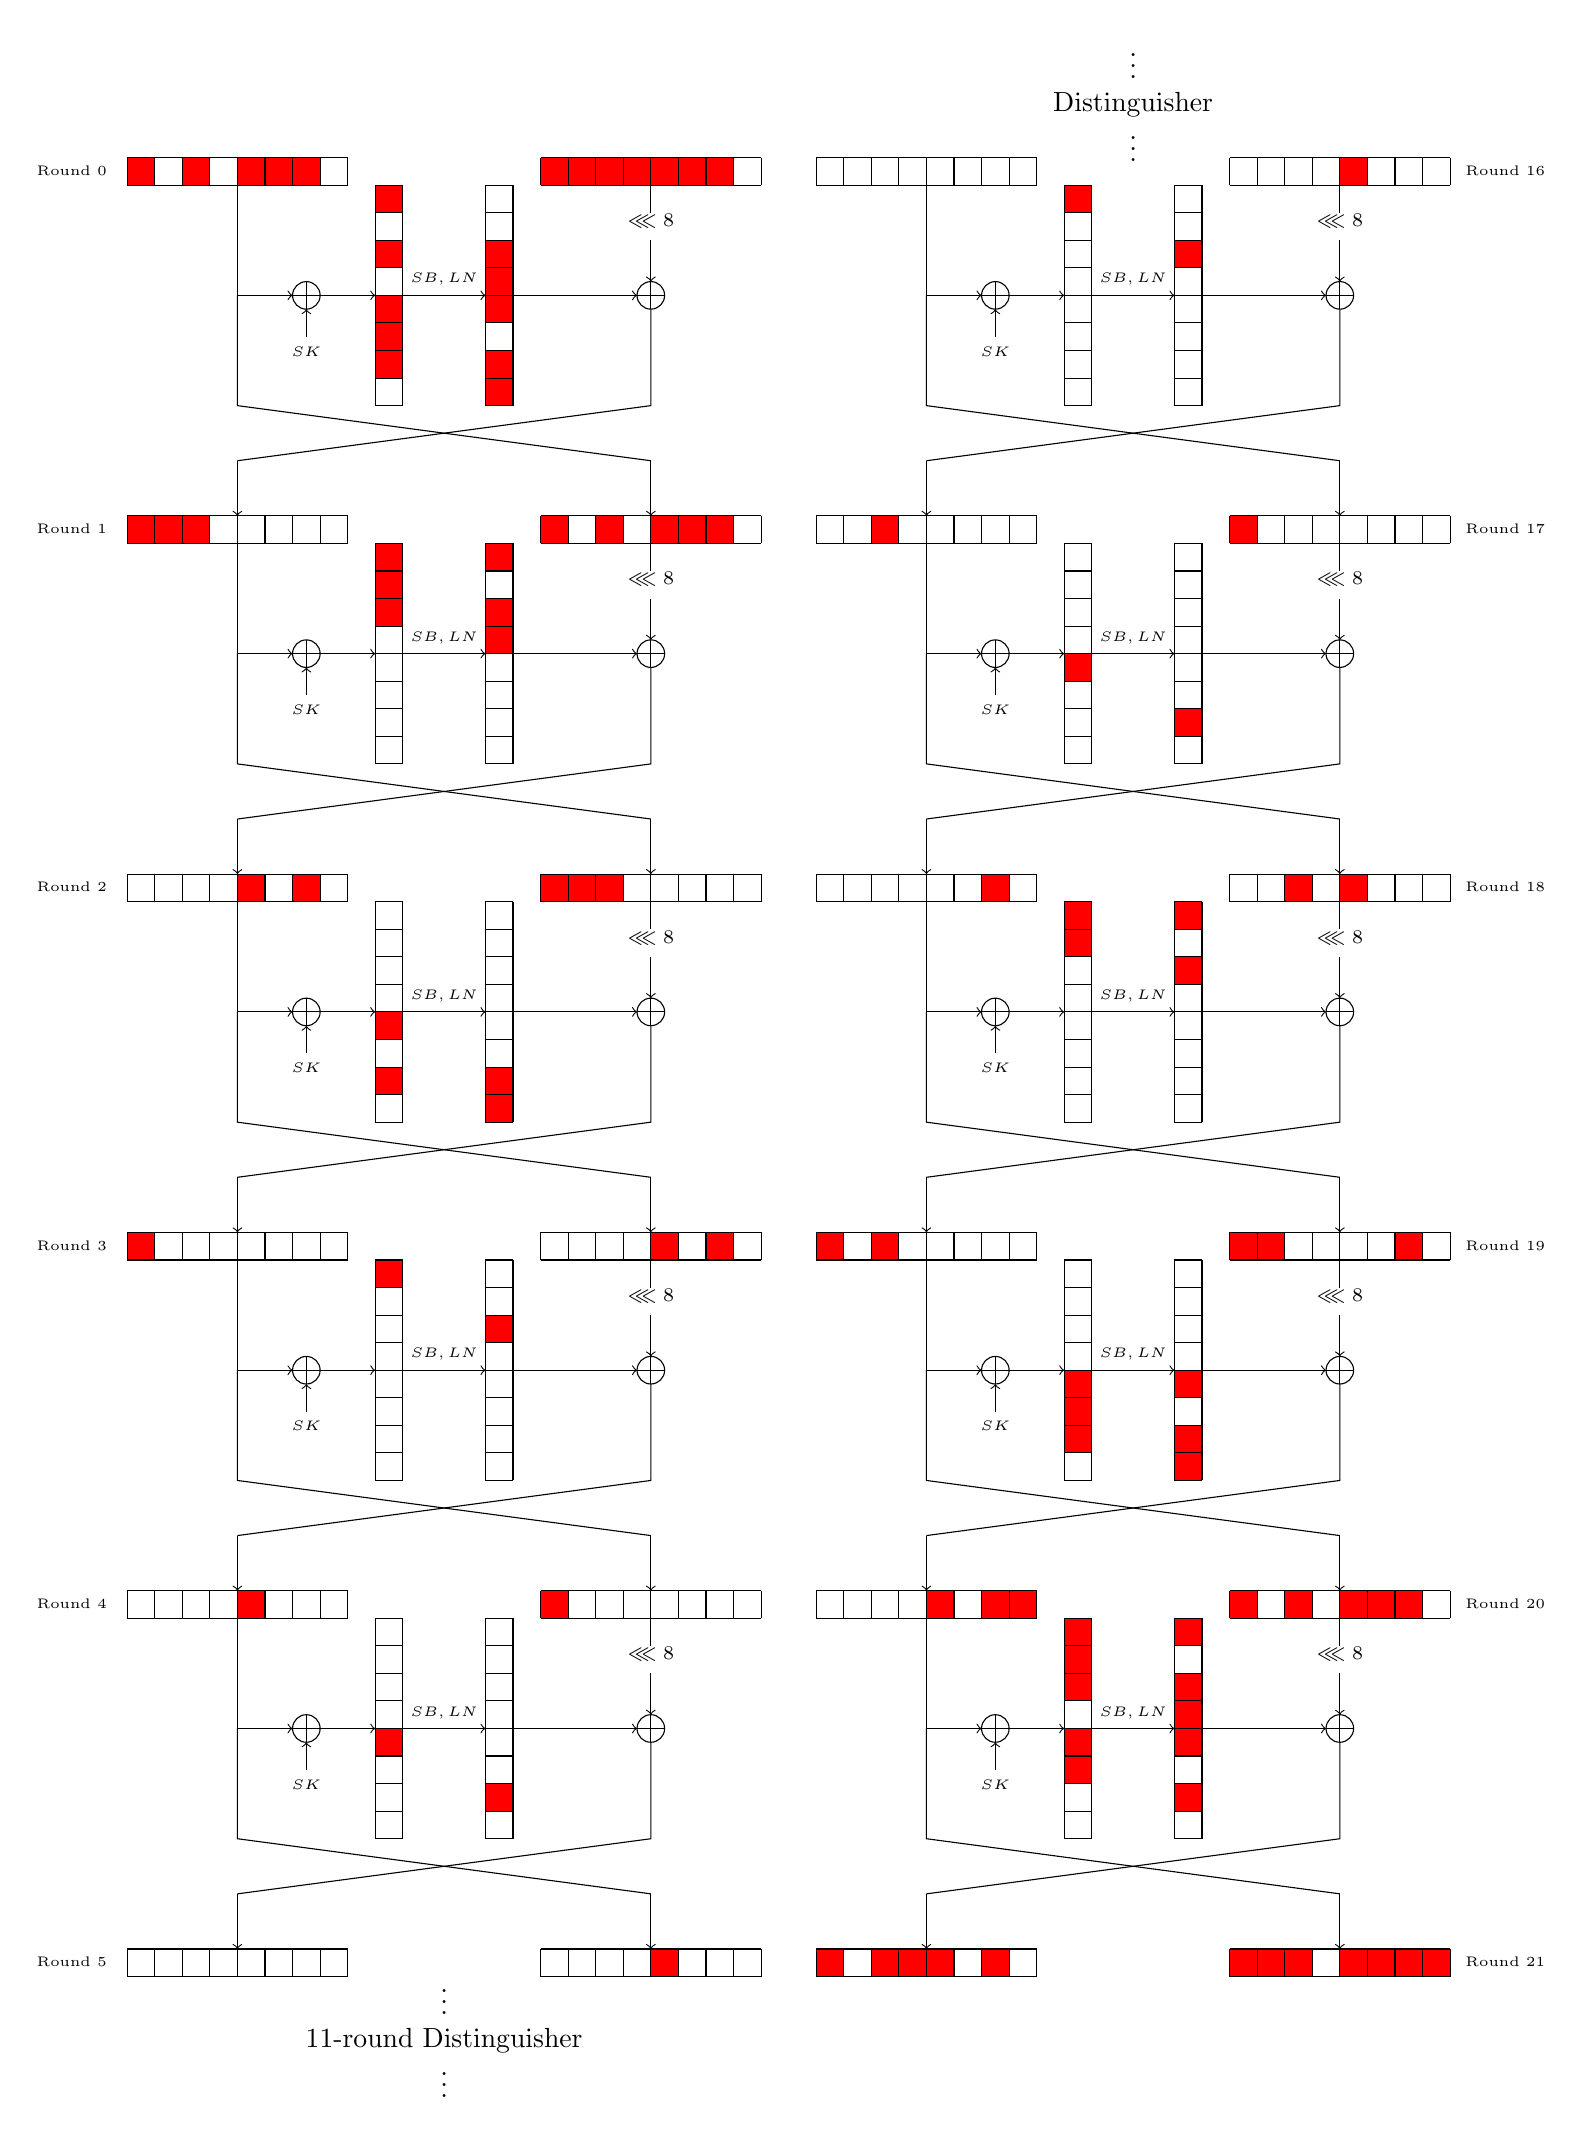
\begin{tikzpicture}[scale=0.35]
\begin{scope}[yshift = -52 cm]
\fill[red] (15,0)rectangle +(1,1);
\fill[red] (4,0)rectangle +(1,1);
\fill[red] (9,-5)rectangle +(1,1);
\fill[red] (13,-7)rectangle +(1,1);
\end{scope}
\begin{scope}[yshift = -39 cm]
\fill[red] (0,0)rectangle +(1,1);
\fill[red] (9,-1)rectangle +(1,1);
\fill[red] (13,-3)rectangle +(1,1);
\fill[red] (19,0)rectangle +(1,1);
\fill[red] (21,0)rectangle +(1,1);
\end{scope}
\begin{scope}[yshift = -26 cm]
\fill[red] (15,0)rectangle +(1,1);
\fill[red] (16,0)rectangle +(1,1);
\fill[red] (17,0)rectangle +(1,1);
\fill[red] (4,0)rectangle +(1,1);
\fill[red] (9,-5)rectangle +(1,1);
\fill[red] (6,0)rectangle +(1,1);
\fill[red] (13,-7)rectangle +(1,1);
\fill[red] (9,-7)rectangle +(1,1);
\fill[red] (13,-8)rectangle +(1,1);
\end{scope}
\begin{scope}[yshift = -13 cm]
\fill[red] (0,0)rectangle +(1,1);
\fill[red] (15,0)rectangle +(1,1);
\fill[red] (13,-1)rectangle +(1,1);
\fill[red] (9,-1)rectangle +(1,1);
\fill[red] (1,0)rectangle +(1,1);
\fill[red] (9,-2)rectangle +(1,1);
\fill[red] (2,0)rectangle +(1,1);
\fill[red] (17,0)rectangle +(1,1);
\fill[red] (13,-3)rectangle +(1,1);
\fill[red] (9,-3)rectangle +(1,1);
\fill[red] (13,-4)rectangle +(1,1);
\fill[red] (19,0)rectangle +(1,1);
\fill[red] (20,0)rectangle +(1,1);
\fill[red] (21,0)rectangle +(1,1);
\end{scope}
\begin{scope}[yshift = 0 cm]
\fill[red] (0,0)rectangle +(1,1);
\fill[red] (15,0)rectangle +(1,1);
\fill[red] (9,-1)rectangle +(1,1);
\fill[red] (16,0)rectangle +(1,1);
\fill[red] (2,0)rectangle +(1,1);
\fill[red] (17,0)rectangle +(1,1);
\fill[red] (13,-3)rectangle +(1,1);
\fill[red] (9,-3)rectangle +(1,1);
\fill[red] (18,0)rectangle +(1,1);
\fill[red] (13,-4)rectangle +(1,1);
\fill[red] (4,0)rectangle +(1,1);
\fill[red] (19,0)rectangle +(1,1);
\fill[red] (13,-5)rectangle +(1,1);
\fill[red] (9,-5)rectangle +(1,1);
\fill[red] (5,0)rectangle +(1,1);
\fill[red] (20,0)rectangle +(1,1);
\fill[red] (9,-6)rectangle +(1,1);
\fill[red] (6,0)rectangle +(1,1);
\fill[red] (21,0)rectangle +(1,1);
\fill[red] (13,-7)rectangle +(1,1);
\fill[red] (9,-7)rectangle +(1,1);
\fill[red] (13,-8)rectangle +(1,1);
\end{scope}
\begin{scope}[yshift = -65 cm]
\fill[red] (19,0)rectangle +(1,1);
\draw (0,0) grid +(8,1);
\draw (15,0) grid +(8,1);
\node[left=20pt,above] at (0,0) {\tiny Round 5};
\node[below,align = center] at(11.5,0.5) {$\vdots$\\ 11-round Distinguisher\\$\vdots$};
\end{scope}
\foreach \x in {0,1,2,3,4}{
\begin{scope}[yshift = -\x*13 cm]
\draw (0,0) node[left=20pt,above]{\tiny Round $\x$} grid +(8,1);
\draw (15,0) grid +(8,1);
\draw[->](4,0)|-+(2,-4);
\draw[->] (6,-4)--+(3,0);
\draw (9,-8) grid +(1,8);
\draw[->] (10,-4)--node[above]{\tiny $SB,LN$} +(3,0);
\draw (13,-8) grid +(1,8);
\draw[->](13,-4)--+(5.5,0);
\draw(19,0)--+(0,-1);
\draw (19,-0.6) node[below = 1pt]{\scriptsize $\lll 8$};
\draw[->] (19,-2)--+(0,-1.5);
\draw (19,-4) circle (0.5);
\draw (18.5,-4)--+(1,0);
\draw(19,-3.5)--+(0,-1);
\draw (6.5,-4) circle (0.5);
\draw[->](6.5,-5.5) -- node[below=5pt]{\tiny $SK$} + (0,1);
\draw (6.5,-3.5)--+(0,-1);
\draw (19,-4.5)--++(0,-3.5)--++(-15,-2);
\draw[->] (4,-10)--+(0,-2);
\draw (4,-4)--++(0,-4)--+(15,-2);
\draw[->](19,-10)--+(0,-2);
\end{scope}

}

\begin{scope}[yshift = 0 cm, xshift = 25 cm]
\fill[red] (9,-1)rectangle +(1,1);
\fill[red] (13,-3)rectangle +(1,1);
\fill[red] (19,0)rectangle +(1,1);
\end{scope}
\begin{scope}[yshift = -13 cm, xshift = 25 cm]
\fill[red] (15,0)rectangle +(1,1);
\fill[red] (2,0)rectangle +(1,1);
\fill[red] (9,-5)rectangle +(1,1);
\fill[red] (13,-7)rectangle +(1,1);
\end{scope}
\begin{scope}[yshift = -26 cm, xshift = 25 cm]
\fill[red] (13,-1)rectangle +(1,1);
\fill[red] (9,-1)rectangle +(1,1);
\fill[red] (9,-2)rectangle +(1,1);
\fill[red] (17,0)rectangle +(1,1);
\fill[red] (13,-3)rectangle +(1,1);
\fill[red] (19,0)rectangle +(1,1);
\fill[red] (6,0)rectangle +(1,1);
\end{scope}
\begin{scope}[yshift = -39 cm, xshift = 25 cm]
\fill[red] (0,0)rectangle +(1,1);
\fill[red] (15,0)rectangle +(1,1);
\fill[red] (16,0)rectangle +(1,1);
\fill[red] (2,0)rectangle +(1,1);
\fill[red] (13,-5)rectangle +(1,1);
\fill[red] (9,-5)rectangle +(1,1);
\fill[red] (9,-6)rectangle +(1,1);
\fill[red] (21,0)rectangle +(1,1);
\fill[red] (13,-7)rectangle +(1,1);
\fill[red] (9,-7)rectangle +(1,1);
\fill[red] (13,-8)rectangle +(1,1);
\end{scope}
\begin{scope}[yshift = -52 cm, xshift = 25 cm]
\fill[red] (15,0)rectangle +(1,1);
\fill[red] (13,-1)rectangle +(1,1);
\fill[red] (9,-1)rectangle +(1,1);
\fill[red] (9,-2)rectangle +(1,1);
\fill[red] (17,0)rectangle +(1,1);
\fill[red] (13,-3)rectangle +(1,1);
\fill[red] (9,-3)rectangle +(1,1);
\fill[red] (13,-4)rectangle +(1,1);
\fill[red] (4,0)rectangle +(1,1);
\fill[red] (19,0)rectangle +(1,1);
\fill[red] (13,-5)rectangle +(1,1);
\fill[red] (9,-5)rectangle +(1,1);
\fill[red] (20,0)rectangle +(1,1);
\fill[red] (9,-6)rectangle +(1,1);
\fill[red] (6,0)rectangle +(1,1);
\fill[red] (21,0)rectangle +(1,1);
\fill[red] (13,-7)rectangle +(1,1);
\fill[red] (7,0)rectangle +(1,1);
\end{scope}
\begin{scope}[yshift = -65 cm, xshift = 25 cm]
\fill[red] (0,0)rectangle +(1,1);
\fill[red] (15,0)rectangle +(1,1);
\fill[red] (16,0)rectangle +(1,1);
\fill[red] (2,0)rectangle +(1,1);
\fill[red] (17,0)rectangle +(1,1);
\fill[red] (3,0)rectangle +(1,1);
\fill[red] (4,0)rectangle +(1,1);
\fill[red] (19,0)rectangle +(1,1);
\fill[red] (20,0)rectangle +(1,1);
\fill[red] (6,0)rectangle +(1,1);
\fill[red] (21,0)rectangle +(1,1);
\fill[red] (22,0)rectangle +(1,1);
\draw (0,0) grid +(8,1);
\draw (15,0) grid +(8,1);
\node[right=20pt,above] at (23,0) {\tiny Round 21};
\end{scope}
\begin{scope}[yshift = -0 cm, xshift = 25 cm]
\node[above,align = center] at(11.5,0.5) {$\vdots$\\Distinguisher\\ $\vdots$};
\end{scope}
\foreach \y in {0,1,2,3,4}{
\begin{scope}[yshift = -\y*13 cm, xshift = 25 cm]
\draw (0,0) grid +(8,1);
\node[right=20pt,above] at (23,0) {\tiny Round \pgfmathparse{int(\y+16)}\pgfmathresult};
\draw (15,0) grid +(8,1);
\draw[->](4,0)|-+(2,-4);
\draw[->] (6,-4)--+(3,0);
\draw (9,-8) grid +(1,8);
\draw[->] (10,-4)--node[above]{\tiny $SB,LN$} +(3,0);
\draw (13,-8) grid +(1,8);
\draw[->](13,-4)--+(5.5,0);
\draw(19,0)--+(0,-1);
\draw (19,-0.6) node[below = 1pt]{\scriptsize $\lll 8$};
\draw[->] (19,-2)--+(0,-1.5);
\draw (19,-4) circle (0.5);
\draw (18.5,-4)--+(1,0);
\draw(19,-3.5)--+(0,-1);
\draw (6.5,-4) circle (0.5);
\draw[->](6.5,-5.5) -- node[below=5pt]{\tiny $SK$} + (0,1);
\draw (6.5,-3.5)--+(0,-1);
\draw (19,-4.5)--++(0,-3.5)--++(-15,-2);
\draw[->] (4,-10)--+(0,-2);
\draw (4,-4)--++(0,-4)--+(15,-2);
\draw[->](19,-10)--+(0,-2);
\end{scope}

}


\end{tikzpicture}
\end{document}